\section{Sequence To Sequence Model} \label{sec:Seq2Seq}

A \textbf{sequence-to-sequence (Seq-to-Seq) model} is often used in natural language processing for \nameref{nlptask:machinetranslationMT}. It takes a sequence of items such as words and outputs another sequence of items. It uses an \textbf{Encoder} that processes the inputs, squashes this information into a \emph{fixed-length} \textbf{context vector}, also known as a \textbf{sentence embedding} or \textbf{thought vector}. The Seq-to-Seq model sends this representation of the source sentence to a \textbf{Decoder} that outputs a target sentence one word at a time, using the context vector (Alammar, 2018a). Commonly, the Encoder and Decoder are \hyperref[sec:RNN]{RNNs} such as \hyperref[sec:LSTM]{LSTMs} or \hyperref[sec:GRU]{GRUs}.


\subsection{Describing Seq-to-Seq Model}

The key feature in the Seq-to-Seq model different from a \hyperref[sec:RNN]{recurrent neural network (RNN)} is the \textbf{context vector}, or the final hidden state of the Encoder. When the Encoder processes the input sequence $\overrightarrow{x} = \{ x_1, ..., x_{T_x} \}$ of individual word vectors $x_t$ in the input sentence $X$, the information is squashed into a \emph{fixed-length} context vector. Formally, a \hyperref[sec:GRU]{gated recurrent unit (GRU)} as the Encoder would output a hidden state given a previous hidden state and the current input: 
$$
h_t = \text{EncoderGRU} \Big( x_t, h_{t-1} \Big)
$$ 
where the context vector named $z$ equals the last hidden state: $z = h_{T_x}$. 
\newline 
The context vector is then passed to the Decoder along with a target token $y_t$ and previous Decoder hidden state $s_{t-1}$ to return a current hidden state, $s_t$:
$$
s_t = \text{DecoderGRU} \Big( y_t, s_{t-1}, z \Big)
$$
The context vector $z$ does not have a time step $t$ subscript, meaning this same context vector from the Encoder is reused each time step in the Decoder. 


\begin{figure}[h]
\vspace{-5pt}
\centering
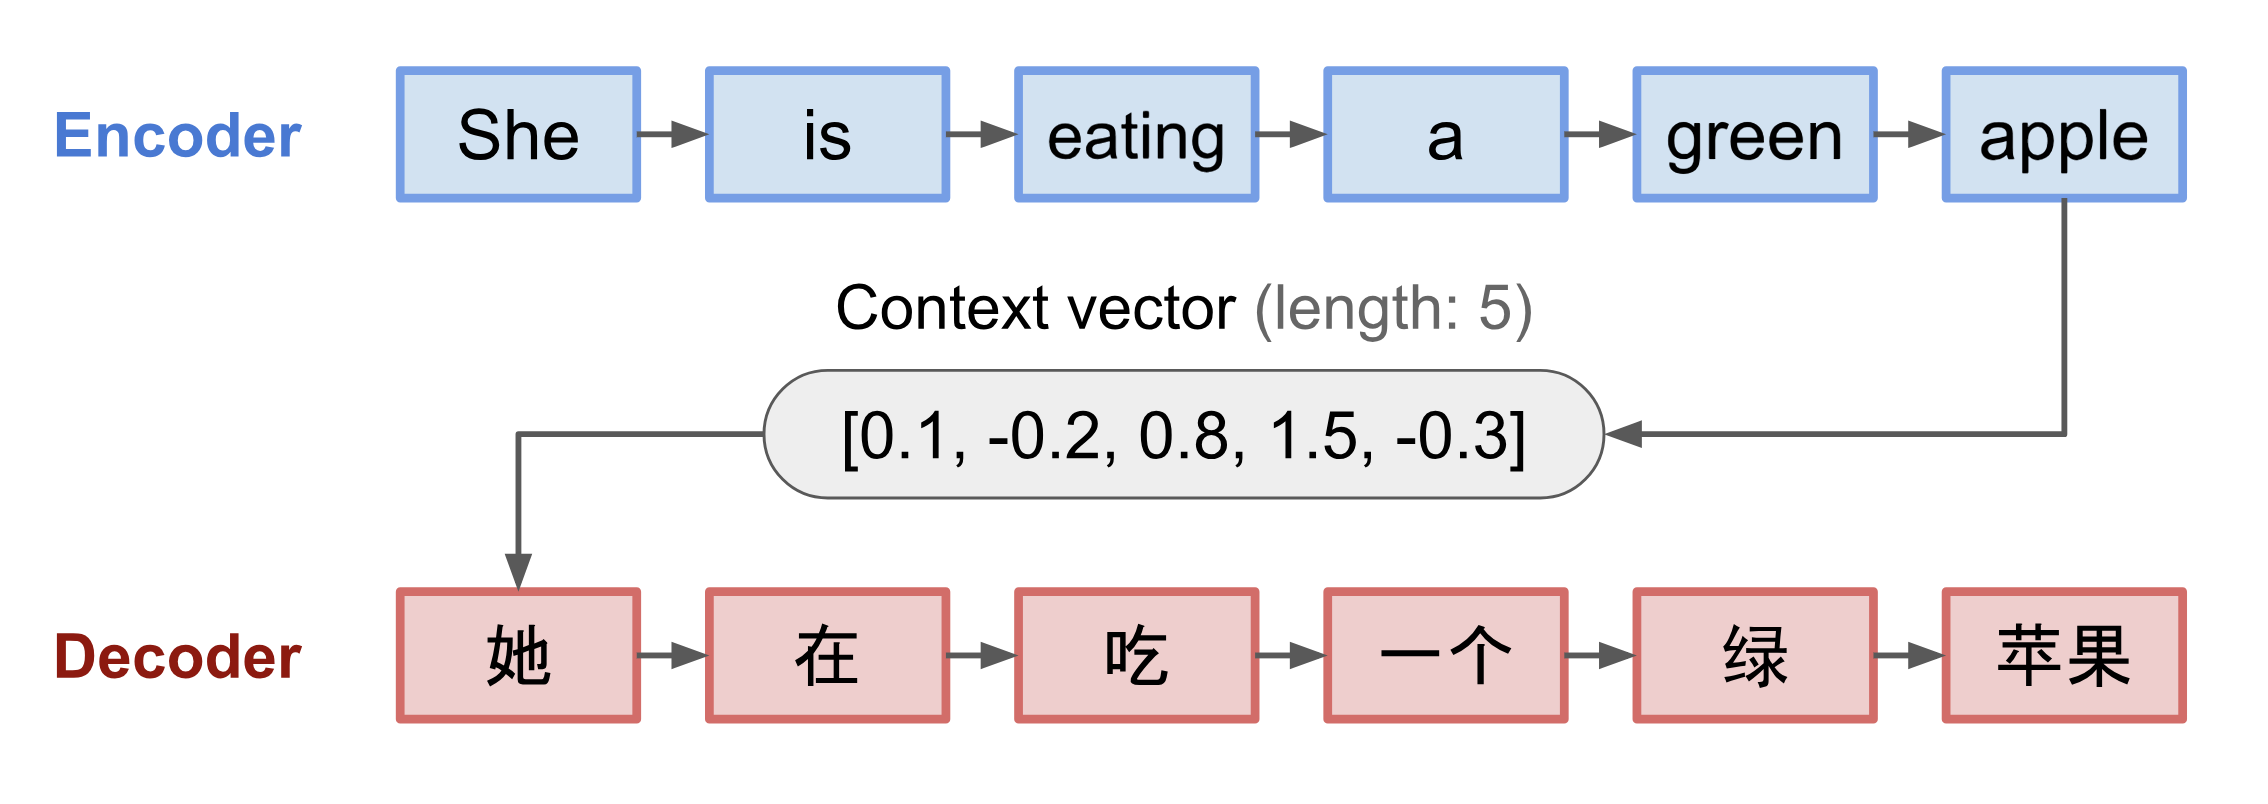
\includegraphics[width=0.6\textwidth]{imgs/seqtoseq_greenapple.png}
\vspace{-5pt}
\caption{\footnotesize Encoder-Decoder with Context Vector in a Seq-to-Seq model, translating the sentence ``She is eating a green apple" to Chinese. From \emph{Attention? Attention!}, by Weng, 2018. \url{https://lilianweng.github.io/lil-log/2018/06/24/attention-attention.html}. Copyright 2018 by Weng.}
\vspace{-5pt}
\end{figure}


\subsection{Problem with Seq-to-Seq Models} \label{sec:ProblemWithSeq2Seq}

Compressing the inputs into such a \textbf{fixed-length} vector leads to a \textbf{long-term dependency problem} since only the last hidden state of the Encoder is used. Thus, the Seq-to-Seq model becomes \textit{\hyperref[sec:ProblemWithRNNs]{incapable of memory}}, similar to  \hyperref[sec:RNN]{RNNs}.

\subsection{The Attention Mechanism} \label{sec:AttentionMechanism}

The \textbf{attention mechanism} was proposed in \nameref{nlptask:neuralmachinetranslationNMT} task to memorize longer sentences by ``selectively focusing on parts of the source sentence" as required (Luong et al., 2015). Instead of creating a single context vector $z$ from the Encoder's last hidden state $h_{T_x}$, the \emph{attention architecture} creates a context vector for each input word or timestep $t$, reducing the information compression problem. This means the attention mechanism uses all the hidden states generated by the Encoder as inputs for the decoding process. For each Decoder output, the attention mechanism ``selectively picks out specific elements from the [input] sequence to produce the [Decoder] output" (Loye, 2019). This essentially creates links between the context vector and entire source input. A general illustration is in \cref{fig:attention}.

\begin{figure}[h]
\centering
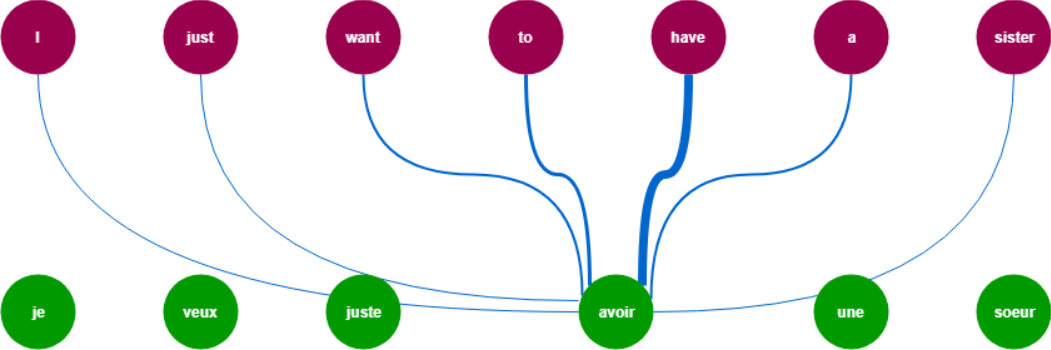
\includegraphics[width=0.6\textwidth]{imgs/attention.png}
\caption{\footnotesize Attention Mechanism: How words are considered for contextual evidence. From \emph{Intuitive Understanding of Seq2seq model and Attention Mechanism in Deep Learning}, by Medium, 2019. \url{https://medium.com/analytics-vidhya/intuitive-understanding-of-seq2seq-model-attention-mechanism-in-deep-learning-1c1c24aace1e}. Copyright n.d by n.d.}
\label{fig:attention}
\end{figure}

\subsection{Seq-to-Seq Model Using Attention}

The key components of a Seq-to-Seq model with attention are its attention \hyperref[sec:ForwardProp]{forward pass}, which computes attention scores, and Decoder \hyperref[sec:ForwardProp]{forward pass}, which outputs the context vector. 

\subsubsection{Forward Pass of Attention}

The attention mechanism is viewed as a layer in the Seq-to-Seq model with a \hyperref[sec:ForwardProp]{forward pass} that updates parameters. The steps for the \hyperref[sec:ForwardProp]{forward pass} to calculate attention scores $\alpha_{ti}$ is as follows: 
\begin{enumerate}
    \item First, an \textbf{alignment model} $\text{align}$ is used to calculate \textbf{energy scores} $e_{ti}$ that measure how well the ``inputs around position $i$ and the output at position $t$ match" (Bahdanau et al., 2016). The energy scores are weights specifying how much of the Decoder hidden state $s_{t-1}$ and the Encoder hidden state $h_i$ of the source sentence should be considered for each output (Ta-Chun, 2018; Bahdanau et al., 2016). 
    $$
    e_{ti} = \text{align} \Big(s_{t-1}, h_i \Big)
    $$ 
    
    \item Next, the energy score $e_{ti}$ is passed through a \hyperref[sec:NeuralLM]{feed-forward neural network} and \hyperref[cnc:softmaxLayer]{softmax} to calculate the attention scores, $\alpha_{ti}$:
    $$
    \alpha_{ti} = \frac{\exp{(e_{ti})} } { \sum_{k=1}^{T_x} \exp{(e_{ik})} }
    $$
    Transforming the energy scores via \hyperref[cnc:softmaxLayer]{softmax} ensures the attention vector $\overrightarrow{\alpha} = \Big \{ \alpha_{ti} \Big \}$ has values normalized between $0$ and $1$. 
\end{enumerate}

%\begin{center}
%    \pythonCodeFile{code/tut3_AttentionClass.py}
%\end{center}

% TODO: line wrapping

\subsubsection{Forward Pass of Decoder}

Once the attention scores have been calculated, the Decoder can calculate the context vector, $c_t$, which is a sum of Encoder hidden states $h_i$ weighted by attention scores $\overrightarrow{\alpha} = \Big \{ \alpha_{ti} \Big \}$ (Ta-Chun, 2018): 
$$
c_t = \sum_{i=1}^{T_x} \alpha_{ti} \cdot h_i
$$

Intuitively, the context vector is an \textbf{expectation}. The attention score $\alpha_{ti}$ is the probability that target word $y_t$ is aligned to (or translated from) an input word $x_j$. Then the $t$-th context vector $c_t$ is the expected hidden state over all hidden states $h_i$ with probabilities $\alpha_{ti}$, where these corresponding energies $e_{ti}$) quantify the importance of Encoder hidden state $h_i$ with respect to the previous Decoder hidden state $s_{t-1}$ in deciding the next Decoder state $s_t$ for generating target word $y_t$. \newline 

Through this attention mechanism in the Decoder, we can relieve the Encoder of the burden of encoding all source sentence information into a fixed-length vector, allowing information to spread through the hidden state sequence $\overrightarrow{h} = \Big \{ h_1,...,h_T\Big \}$ and later be retrieved by the Decoder (Trevett, 2020). \newline

%\begin{center}
%    \pythonCodeFile{code/tut3_DecoderClass.py}
%\end{center}


\subsubsection{Forward Pass of Seq-to-Seq Model}

Finally, the Seq-to-Seq model can use the Encoder, Decoder and attention in conjunction. Its \hyperref[sec:ForwardProp]{forward pass} is (Trevett, 2020): 
\begin{enumerate}
    \item Create an output tensor to hold predicted words $\hat{y}$
    
    \item Pass the source sequence $\overrightarrow{x} = \Big \{ x_1, ..., x_T \Big \}$ into the Encoder to receive the contexts $\overrightarrow{z}$ alongside the hidden states $\overrightarrow{h} = \Big \{ h_1, ..., h_T \Big \}$.
    
    \item Set equal the initial Decoder hidden state $s_0$ and last Encoder hidden state $h_T$.
    
    \item Decode within a loop: insert the target token $y_t$ and previous hidden state $s_t$ and all Encoder outputs $\overrightarrow{h}$ into the Decoder to get a prediction $\hat{y}_{t+1}$ and new hidden state $s_t$.
    
    
\end{enumerate}

As an application of the Seq-to-Seq model with attention to \nameref{nlptask:neuralmachinetranslationNMT}, PyTorch code with explanations can be found in \nameref{app:Appendix_Seq2Seq}
%\begin{center}
%    \pythonCodeFile{code/tut3_Seq2Seq.py}
%\end{center}